99.\begin{figure}[ht!]
\center{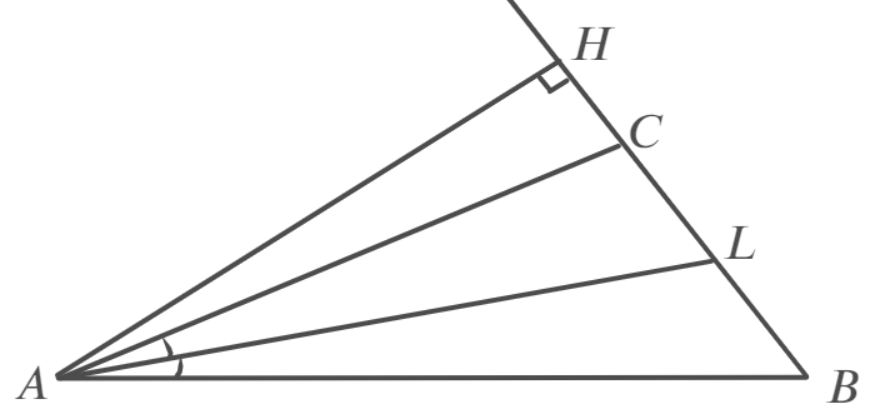
\includegraphics[scale=0.35]{g99.png}}
\end{figure}\\
Пусть $\angle A=2x,\ \angle B=5x,\ \angle C=11x,$ тогда $2x+5x+11x=180^\circ,\ 18x=180^\circ,\ x=10^\circ,\ \angle A=20^\circ,\ \angle C=110^\circ.$ Так как $\angle C>90^\circ,$ высота упадёт наружу и  $\angle ACH=180^\circ-110^\circ=70^\circ,\ \angle HAC=90^\circ-70^\circ=20^\circ.$ Таким образом, $\angle HAL=\angle HAC+\angle CAL=20^\circ+20^\circ:2=30^\circ.$
ewpage

oindent100. \begin{figure}[ht!]
\center{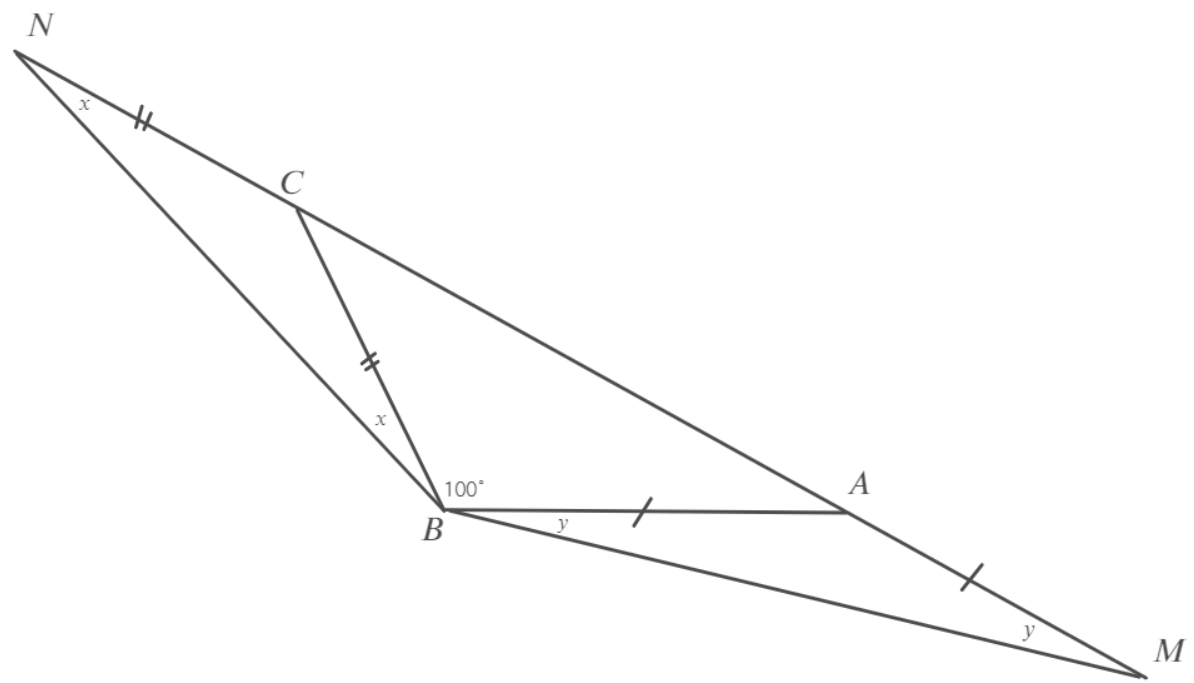
\includegraphics[scale=0.35]{g100.png}}
\end{figure}\\
Треугольники $NCB$ и $MAB$ равнобедренные, пусть $\angle CNB=\angle CBN=x,\ \angle AMB=\angle ABM=y.$ Тогда как внешние углы $\angle C=2x,\ \angle A=2y$ и из треугольника $ABC:\ 2x+2y+100^\circ=180^\circ,\ x+y=40^\circ,$ значит $\angle MBN=100^\circ+40^\circ=140^\circ.$\\
